\documentclass{article}
\usepackage[backend=biber, style=apa]{biblatex}
\usepackage{hyperref}
\usepackage{graphicx} % Required for inserting images
\usepackage{amsmath}
\usepackage{amssymb}
\usepackage{enumitem}
\usepackage{geometry}
\usepackage{wrapfig}

\usepackage[table,xcdraw]{xcolor}

\geometry{margin=1in}\addbibresource{references_find.bib}
\setlength{\intextsep}{0pt} 


\title{Findings}
\author{Anton Mukin}
\date{\today}

\setlength{\parindent}{0pt}


\begin{document}

\maketitle

\subsection{Abstract}

\subsection{Introduction}
This project started with a simple Idea -- A calculator that rather than 
working systematically, predicts your answer using a neural network. The 
question which neural network architecture would fit this job best is what 
what truly propelled this project.

This document presents the findings, which have been learned with the 
project: A Predictive Calculator.

\subsection{Feed-forward Neural Networks (FNNs)}
Since the functionality of a FNN has already been discussed in the 
literature study, were mentioned in the methodology document and no new 
information on FNNs has been found since then by the author, this topic 
will not be discussed in this document. 

Though, FNNs will make an appearance later on in this document.

\newpage
\tableofcontents
\newpage

\section{RNN}

Recurrent Neural Networks (RNNs) work similar to FNNs with one key 
difference: There is a vector called the hidden-state. This vector contains 
information about previous inputs. The hidden-state of the previous 
time-step, in addition to the input of the current time-step, is fed into a 
model which computes the hidden-state of the present time-step. The output 
of each time-step is calculated by feeding the respective hiddenstate to a 
model.


\subsection{Numerical Visualization of a RNN:}
Let:
\begin{itemize}
    \item $x_t$: Input at time step $t$
    \item $h_t$: Hidden state at time step $t$
    \item $y_t$: Output at time step $t$
    \item $W_{xh}$: Weight matrix connecting input to hidden state
    \item $W_{hh}$: Weight matrix connecting previous hidden state to current hidden state (recurrent weights)
    \item $W_{hy}$: Weight matrix connecting hidden state to output
    \item $b_h$: Bias vector for the hidden layer
    \item $b_y$: Bias vector for the output layer
    \item $\sigma$: Activation function (in our case: PReLU)
    \item $\sigma_{out}$: Activation function for the output (linear for regression)
\end{itemize}



$$h_t = \sigma(W_{xh}x_t + W_{hh}h_{t-1} + b_h)$$

$$y_t = \sigma_{out}(W_{hy}h_t + b_y)$$

\subsection{Relevant Takeaway}
For us this means, the RNN doesn't process an expression as a whole, but 
rather one part after another.
Also, because of how the formula works, Tokens, which are later in the 
sequence, play a more impactful role on the models prediction, than earlier 
tokens. This means the output number will almost always be closer to the 
last number of the expression, than the first.

This is a common issue with RNNs, not only prevelant in this project. It is 
more widely known as the vanishing gradient problem.

\section{Other Types of RNNs}
To solve the problem described above, different methods have been adopted 
like for example the Long Short-Term Memory (LSTM) proposed by \cite{6795963}, 
the Gated Recurrent Unit (GRU) proposed by \cite{cho2014propertiesneuralmachinetranslation} 
or later even the concept of attention proposed by \cite{bahdanau2016neuralmachinetranslationjointly}.
%https://www.geeksforgeeks.org/deep-learning/rnn-vs-lstm-vs-gru-vs-transformers

\subsection{ Long Short-Term Memory (LSTM)}
The LSTM architecture solves the gradient vanishing problem by using a memory 
cell. The model can use this to store \eqref{eq:cell_update_lstm}, forget 
\eqref{eq:forget_gate_lstm} and pass information from the 
memory cell to the hidden state \eqref{eq:hidden_state_lstm}.

Let: 
\begin{itemize}
    \item $\sigma(\cdot)$ denotes the sigmoid activation function,
    \item $\tanh(\cdot)$ is the hyperbolic tangent function,
    \item $\odot$ represents element-wise (Hadamard) multiplication,
    \item $[h_{t-1}, x_t]$ is the concatenation of the previous hidden state $h_{t-1}$ and the current input $x_t$,
    \item $W_f, W_i, W_C, W_o$ are trainable weight matrices,
    \item $b_f, b_i, b_C, b_o$ are trainable bias vectors,
    \item $C_t$ is the current memory cell state,
    \item $\tilde{C}_t$ is the candidate cell state,
\end{itemize}

\begin{align}
    % Forget gate
    f_t &= \sigma\!\left(W_f \cdot [h_{t-1}, x_t] + b_f\right) \label{eq:forget_gate_lstm} \\
    % Input gate
    i_t &= \sigma\!\left(W_i \cdot [h_{t-1}, x_t] + b_i\right) \label{eq:input_gate_lstm} \\
    % Candidate cell state
    \tilde{C}_t &= \tanh\!\left(W_C \cdot [h_{t-1}, x_t] + b_C\right) \label{eq:candidate_cell_state_lstm} \\
    % Output gate
    o_t &= \sigma\!\left(W_o \cdot [h_{t-1}, x_t] + b_o\right) \label{eq:output_gate_lstm}\\    
    % Cell state update
    C_t &= f_t \odot C_{t-1} + i_t \odot \tilde{C}_t \label{eq:cell_update_lstm}\\
    % Hidden state (output)
    h_t &= o_t \odot \tanh(C_t) \label{eq:hidden_state_lstm}
\end{align}
Source for the equations: \cite{geeksforgeeks_lstm}
\\[2em]
In the equations you can see the forget gate activation \eqref{eq:forget_gate_lstm}, 
the input gate activation \eqref{eq:input_gate_lstm}, the candidate cell state 
\eqref{eq:candidate_cell_state_lstm} and the output gate activation \eqref{eq:output_gate_lstm}.

The cell state is calculated in \eqref{eq:cell_update_lstm}. There, the forget 
gate which scales the previous cell state is combined with the input gate.

The hidden state is calculated in \eqref{eq:hidden_state_lstm}, where the output 
activation is applied to the cell state.

\subsection{Gated Recurrent Unit (GRU)}

The GRU architecture works in a similar way to the LSTM. Instead of utilizing 
memory cells, they directly use the hiddenstate.

Let:
\begin{itemize}
    \item $\sigma(\cdot)$ is the sigmoid activation function,
    \item $\tanh(\cdot)$ is the hyperbolic tangent function,
    \item $\odot$ denotes element-wise (Hadamard) multiplication,
    \item $[h_{t-1}, x_t]$ is the concatenation of the previous hidden state and current input,
    \item $W_z, W_r, W_h$ are trainable weight matrices,
    \item $b_z, b_r, b_h$ are trainable bias vectors,
    \item $\tilde{h}_t$ is the candidate hidden step
    \item $h_t$ is the current hiddenstep
\end{itemize}

\begin{align}
    % Update gate
    z_t &= \sigma\!\left(W_z [h_{t-1}, x_t] + b_z\right) \label{eq:update_gate_gru} \\
    % Reset gate
    r_t &= \sigma\!\left(W_r [h_{t-1}, x_t] + b_r\right) \label{eq:reset_gate_gru} \\
    % Candidate hidden state
    \tilde{h}_t &= \tanh\!\left(W_h [r_t \odot h_{t-1}, x_t] + b_h\right) \label{eq:candidate_hidden_state_gru} \\
    % Final hidden state
    h_t &= (1 - z_t) \odot h_{t-1} + z_t \odot \tilde{h}_t \label{eq:update_hidden_state_gru}
\end{align}
Source for the equations: \cite{geeksforgeeks_gru}
\\[2em]
Above you can see the update gate activation \eqref{eq:update_gate_gru}, as well 
as the reset gate activation \eqref{eq:reset_gate_gru}.

Further down, the reset gate activation is applied to the previous hidden step 
to calculate the candidate hidden state \eqref{eq:candidate_hidden_state_gru}. 

Lastly the hidden step can be calculated by applying (1 - the update gate 
activation) to the previous hidden step and combining it with the update gate 
activation applied to the hidden state candidate \eqref{eq:update_hidden_state_gru}. 
Depending on whether the update gate activation is larger or smaller, the 
previous hidden step or the candidate hiddenstate will weigh in more on the 
current hidden step.

\subsection{Bidirectional LSTM with Attention}

An architecture of this type consists in part of a bidirectional LSTM, meaning 
two LSTMs working in parallel, one of who process data from front to back, the 
other from back to front, their results are afterwards concatenated together 
and passed on.
\\[2em]
The other part of this architecture is the attention mechanism. Here it is, as 
described by \cite{bahdanau2016neuralmachinetranslationjointly}.

Let:
\begin{itemize}
    \item $\mathbf{h}_t \in \mathbb{R}^{128}$ are the hiddenstates for each 
    timestep $t$, the output from the bidirectional LSTM,
    \item $\mathbf{W} \in \mathbb{R}^{128 \times 128}$ is a trainable weight 
    matrix,
    \item $\mathbf{b} \in \mathbb{R}^{128}$ is a bias vector,
    \item $\mathbf{u} \in \mathbb{R}^{128}$ is a trainable context vector.
\end{itemize}

For each time step $t$, compute:
\begin{align}
    \mathbf{v}_t &= \tanh\!\left( \mathbf{W} \mathbf{h}_t + \mathbf{b} \right) \label{eq:v_bahdanau} \\
    e_t &= \mathbf{u}^\top \mathbf{v}_t \label{eq:attention_score}
\end{align}

Normalize scores using softmax:
\begin{equation}
    \alpha_t = \frac{\exp(e_t)}{\sum_{j=1}^{T} \exp(e_j)} \label{eq:alpha_score}
\end{equation}
The attention weights $\boldsymbol{\alpha} = [\alpha_1, \dots, \alpha_T]$ 
indicate the importance of each time step.

Then compute the context vector:
\begin{equation}
    \mathbf{c} = \sum_{t=1}^{T} \alpha_t \mathbf{h}_t \label{eq:attention_context}
\end{equation}

Source for equations: \cite{cristina_2023_bahdanau}
\\[2em]
An attention score is calculated for each timestep in \eqref{eq:v_bahdanau}, 
\eqref{eq:attention_score}, it is then normalized \eqref{eq:alpha_score}. 
Finally the attention weights scale their respective hiddenstates from the 
LSTMs, to compute the context vector \eqref{eq:attention_context}.

\section{Transformers} \label{sec:transformers}

The best performing and widely used on most tasks to date are transformer 
architectures, they formed the basis for LLM's.

The key to their success: multi-head self-attention.
\\[2em]
In this document we will discuss the transformer architecture as first proposed 
by \cite{vaswani2023attentionneed}.
\subsection{Multi-Head Self-Attention}

\begin{figure}[htbp]
    \centering
    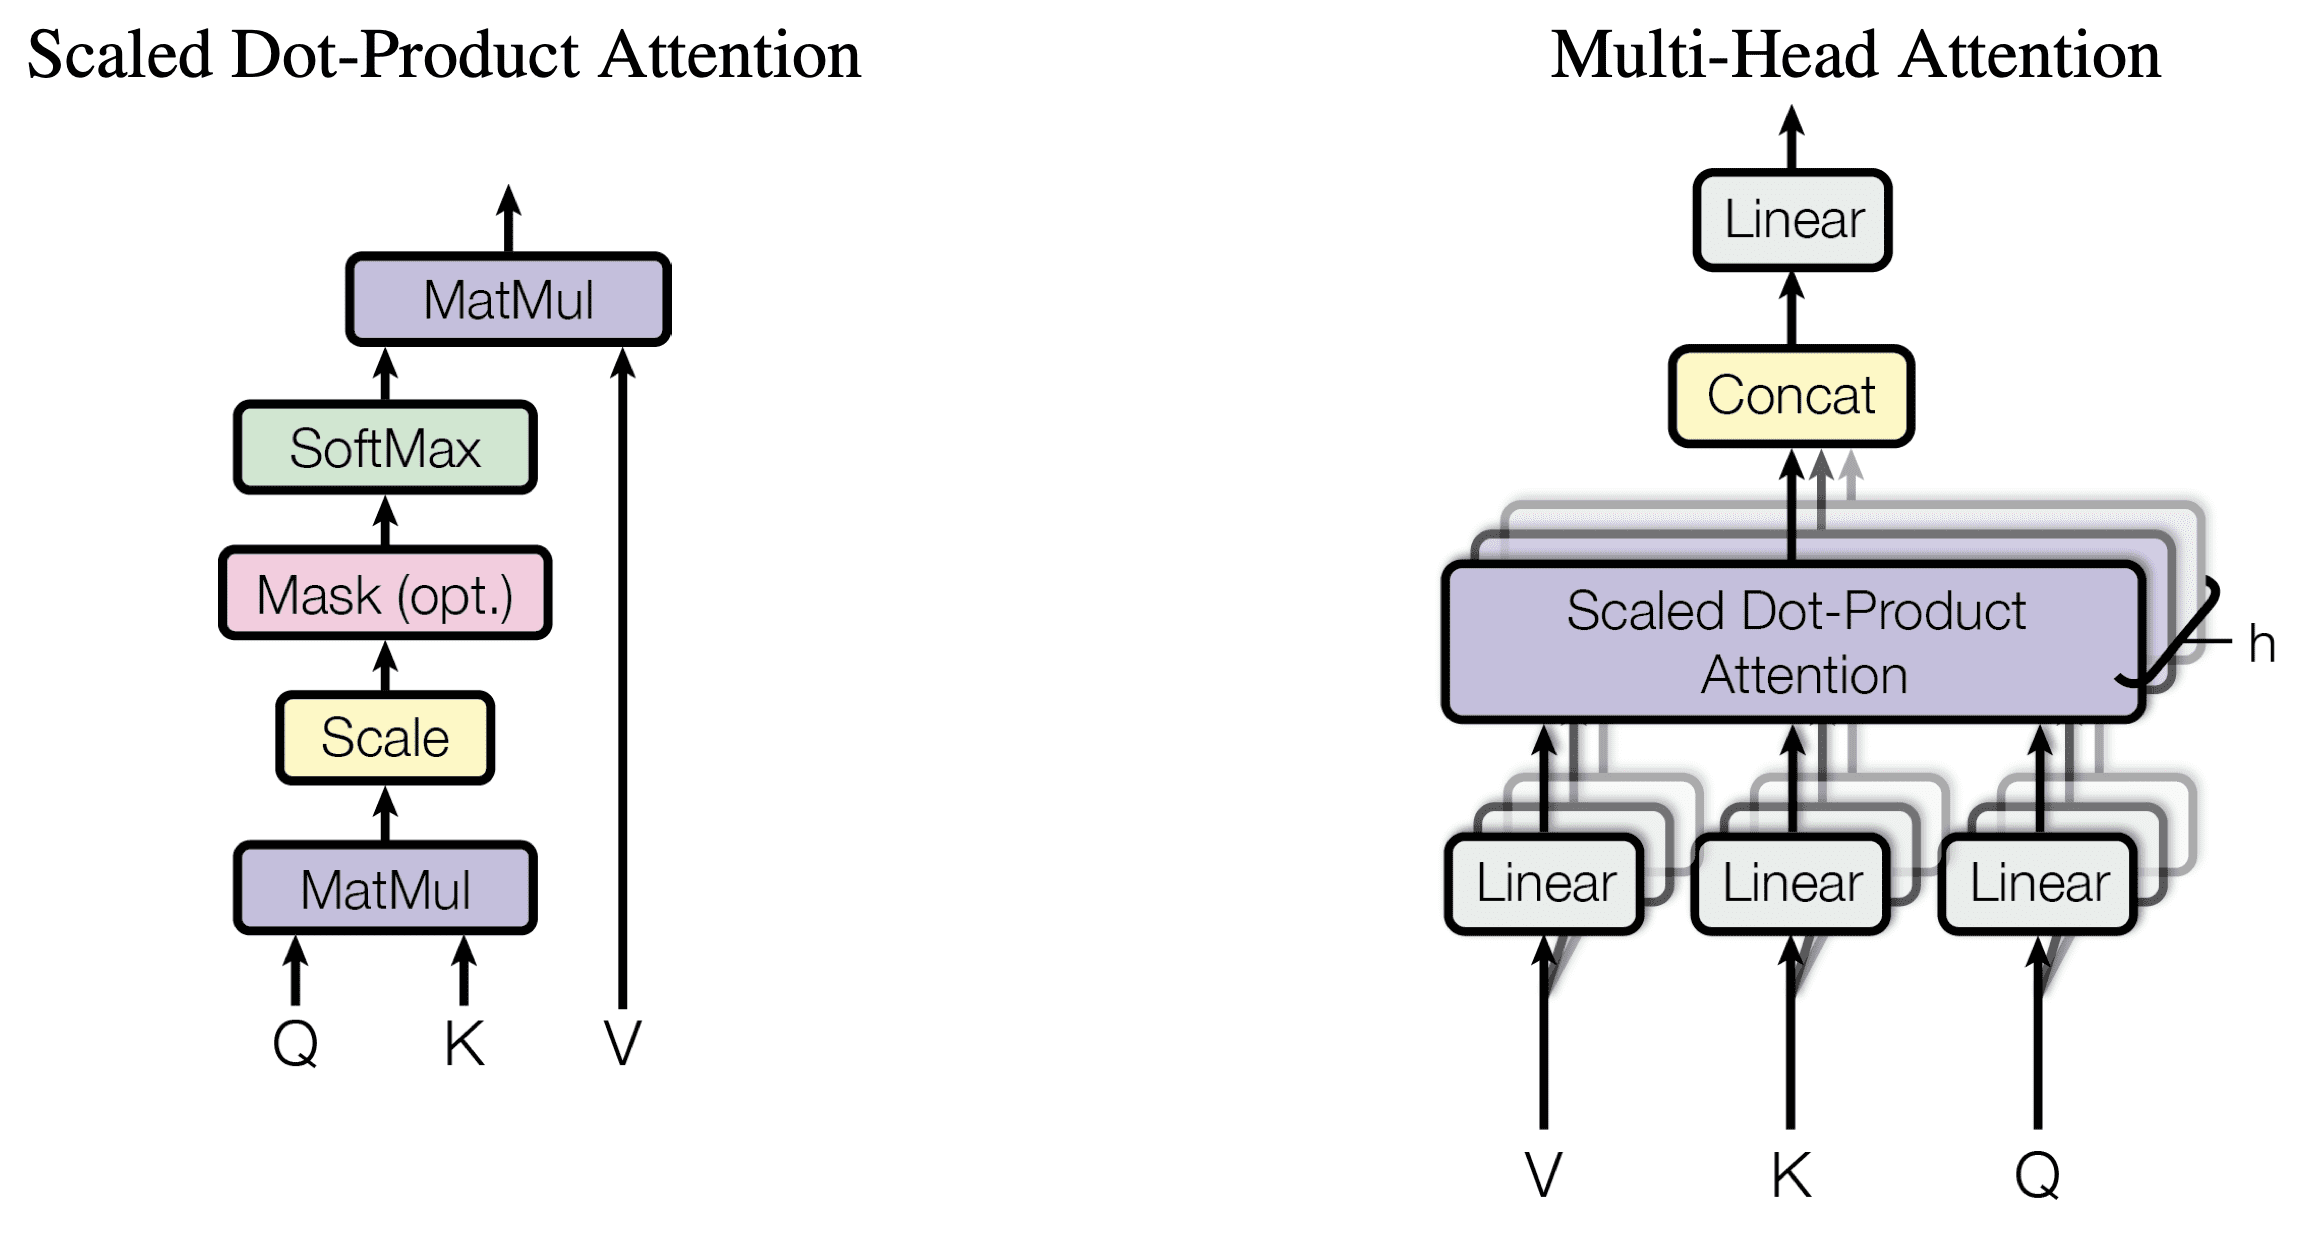
\includegraphics[width=0.5\paperwidth]{images/dotproduct_1.png}
    \caption{Two diagrams from \cite{vaswani2023attentionneed} with the scaled 
    dot-product attention described on the left and multi-head attention on the 
    right.}
    \label{fig:MHAttention}
\end{figure}

Data is first split up eqally into multiple heads which will process it in 
parallel. There, the tensors are linearly projected with trainable weights, 
to obtain queries (Q), keys (K) and values (V) which you can see at the bottom 
of the image.
$$
Q = X W_Q, \quad K = X W_K, \quad V = X W_V
$$
Afterwards, the dot-product between the queries and the keys is calculated and 
scaled\footnote{According to \cite{vaswani2023attentionneed} this is done to 
counteract dot-products growing too large and later overwhelming the softmax 
function.} to determine how simmilar they are. This leaves us with a 
number between 0 and 1 representing how much attention you have to pay. The 
value $V$ represents the actual information of the token we just calculated the 
attention for. This means our final step is to scale the value $V$ by it's 
attention. Pay attention to the equation below. \eqref{eq:sdpAttention}
\begin{equation}
    \text{Attention}(Q, K, V) = \text{softmax}\left( \frac{Q K^\top}{\sqrt{d_k}} \right) V \label{eq:sdpAttention}
\end{equation}

This is done across all heads in parallel. The results are then concatenated\footnote{
This means the are assembled or added back together, to have the same 
dimensions as before they were split up.} back together and they undergo 
a linear projection. As described below:

\begin{gather*}
\text{MultiHead}(Q, K, V) = \text{Concat}(\text{head}_1, ..., \text{head}_h) W^O \\
\text{where: } \text{head}_i = \text{Attention}(Q W_i^Q, K W_i^K, V W_i^V)
\end{gather*}

\newpage
\subsection{The Encoder Layer}

\begin{wrapfigure}{l}{0.3\textwidth}
    \centering
    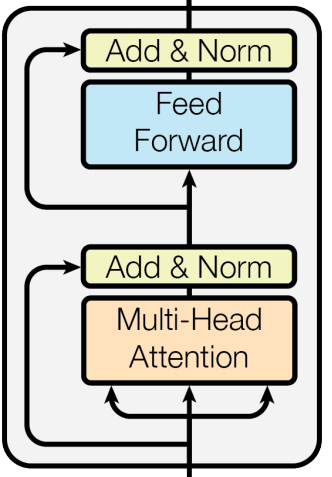
\includegraphics[width=0.2\paperwidth]{images/encodingLayer.png}
    \caption{Encoder Layer as described by \cite{vaswani2023attentionneed}}
    \label{fig:encodingLayer}
\end{wrapfigure}

In figure \ref{fig:encodingLayer} the multi-head attention first undergoes 
a residual connection as well as a layer normalization \footnote{Given an input 
vector, layer normalization works by normalizing it's features and making it so 
their mean is 0.}, as described below:

\begin{gather}
    \text{where Sublayer(x) is the function the residual connection is formed 
    around:} \nonumber \\
    \text{Output}(x) = \text{LayerNorm}\bigl(x + \text{Sublayer}(x)\bigr) \label{eq:ResConnect}
\end{gather}

Afterwards, all tokens are fed into a point-wise FNN, where they are processed 
separately and independently. This part is crucial, to introduce non-linearity 
into the system, as multi-head attention is linear, and non-linearity is needed 
for a model to be able to learn.

\subsection{Point-wise Feed-Forward Network}


Equation \eqref{eq:pointwiseFNN} and figure \ref{fig:pointwiseFNN}:

The pointwise FNN works by taking in a number of $d\_model$ tokens, then a 
layer with a number of $d\_FNN$ neurons with weights and biases $W_1$ and $b_1$ 
is applied to them individually. The activation function ReLU discards all 
negative vlaues and the output layer with weights and biases $W_2$ and $b_1$ 
resets the data back to it's original dimensionality.

After undergoing a residual connection and layer normalization like after 
multihead attention \eqref{eq:ResConnect}, this makes up a single layer of the 
Encoder.

A regressive transformer model, like the one used in this project, consists of 
multiple such encoding layers and last but not least a FNN with a single neuron, 
which works as the output layer.

\begin{equation}
    \text{pointwiseFNN}(x) = \max\bigl(0, \, x W_1 + b_1 \bigr) W_2 + b_2 \label{eq:pointwiseFNN}
\end{equation}

\begin{figure}[htbp]
    \centering
    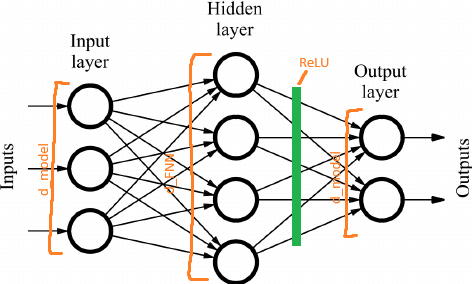
\includegraphics[width=0.4\paperwidth]{images/pointwiseFNN.png}
    \caption{A diagram representing the structure of a pointwise FNN. \href{https://datascience.stackexchange.com/questions/68020/what-is-the-feedforward-network-in-a-transformer-trained-on}
    {source for figure}}
    \label{fig:pointwiseFNN}
\end{figure}

\subsection{Positional Encoding}

Something, that's special about the tranformer, is the fact that data is passed 
through it as a whole. This means the model doesn't have positional understanding 
on it's own. To counteract this effect, a positional encoding is applied to the 
input sequences after the tokenizer.

\newpage
\section{Fine-Tuned Pre-Trained LLMs}

The last model type used for this project are fine-tuned Large 
Language Models (LLMs).
For sources and further reading on this section see (in chronological order; 
left to right): \cite{geeksforgeeks_2024,Stryker_LLM,srinivasan2024transformer,Bergmann_Fine_Tuning}


\subsection{LLM}

LLMs adopt the transformer architecture\footnote{The transformer architecture 
discussed in the previous section \ref{sec:transformers}. It not only consists 
but also a decoder, which is responsible for the model's output} and adapt it 
to imense sizes, by increasing the architecture's hyperparameters, as well as 
employing new technological advancements. The number of parameters used by a 
LLM varies from model to model, but lies in the hundreds of billions per 
popular high-end LLM.

The large size allows large architectures to excell at complicated tasks like 
mostly Natural Language Processing (NLP).

To facilitate, training and predicting on such large architectures, massive super-
computers are used, consisting of thousands of GPUs. They mainly work by utilizing 
parallel processing to distribute the load across multiple powerful GPUs. 

While by far not a super-computer, a tiny replica was used for this project: 
The Nvidia Jetson Orin Nano Super Developer Kit.


\subsection{Fine-Tuning Process}

Most of the time LLMs are trained on huge dumps of unlabeled data, which 
we call unsupervised, or on unlabelled data from which ground truth can be 
inferred, which we call self-supervised data. 

The fine-tuning process on the other hand is mostly done on smaller datasets 
with supervised data, meaning it is labeled.
\\[2em]
In fine-tuning a pre-trained model, with all of it's weights and biases being 
set to an optimized value after the training, is trained again on additional 
data. This will mean, that the models weights will move and change by a little 
amount from the state it was in before fine-tuning. The optimizer will find a 
new minima in which the model will have learned additional information from the 
fine-tuning train-data. When evaluated on test-data the newly fine-tuned model 
should now perform better, than it's pre-trained basemodel counterpart.

\subsection{In Addition}
Please note that these are not regression models, but sequence to sequence 
models, which means that inside the model tokens are processed, not numbers, 
like in the other models discussed. 

For the task in this project Specifically, fine-tuned models will not output a 
float number, but rather an integer, because tokens for floats haven't been 
created. It is the reason why the only metric that makes sense for these models 
is accuracy, which essentially evaluates how many times the model predicted 
correctly.

\newpage

\section{Final Evaluation and Conclusion}

Lastly, the most noteworthy architectures were evaluated and scored on a 
benchmark. The results were documented in this table: 
\\[0.5em]

% Please add the following required packages to your document preamble:
% \usepackage[table,xcdraw]{xcolor}
% Beamer presentation requires \usepackage{colortbl} instead of \usepackage[table,xcdraw]{xcolor}
\begin{table}[htbp]
\begin{tabular}{|lr|r|r|r|r|r|}
\hline
\multicolumn{2}{|l|}{Regression models:}                              & \multicolumn{1}{l|}{FNN2} & \multicolumn{1}{l|}{RNN2} & \multicolumn{1}{l|}{Bidirectional   LSTM\footnote{with bahdanau attention mechanism}} & \multicolumn{1}{l|}{transformer5} & \multicolumn{1}{l|}{transformer 4} \\ \hline
\multicolumn{2}{|l|}{Total   Parameters:}                             & 6’211                     & 222’464                   & 19’535                                    & 1’494’724                         & 114’628                            \\
\multicolumn{2}{|l|}{Architecture   Parameters:}                      & 6’211                     & 222,464                   & 6’511                                     & 498’241                           & 38’209                             \\
\multicolumn{2}{|l|}{Optimizer   Parameters:}                         & -                         &                           & 13’024                                    & 996’483                           & 76’419                             \\
\rowcolor[HTML]{F7C7AC} 
MAE in Range:                              &                          & 0.0389406                 & 0.2730647                 & 0.5908327                                 & 0.0381983                         & 0.0448075                          \\
\rowcolor[HTML]{F7C7AC} 
MRE in Range:                              &                          & 0.0155504                 & 0.1135200                 & 0.2712299                                 & 0.0151836                         & 0.0188047                          \\
\rowcolor[HTML]{94DCF8} 
MAE out Range:                             &                          & 2.2301364                 & 3.5727410                 & 3.2350100                                 & 4.9287004                         & 4.5702314                          \\
\rowcolor[HTML]{94DCF8} 
MRE out Range:                             &                          & 0.2509270                 & 0.3472042                 & 0.3404062                                 & 0.5431157                         & 0.5201459                          \\
\rowcolor[HTML]{FFDC6D} 
\multicolumn{2}{|l|}{\cellcolor[HTML]{FFDC6D}MAE   long Expressions:} & 6.2929916                 & 6.0766930                 & 2.7806435                                 & 6.0680327                         & 6.1630590                          \\ \hline
\rowcolor[HTML]{D86DCD} 
\multicolumn{2}{|l|}{\cellcolor[HTML]{D86DCD}Benchmark   score:}      & 6.6345832                 & 0.4793787                 & 1.7374969                                 & 5.2896368                         & 2.8882827                          \\ \hline
\end{tabular}
\end{table}

And the fine-tuned Language Models, evaluated on their accuracy:
\\[0.5em]

% Please add the following required packages to your document preamble:
% \usepackage[table,xcdraw]{xcolor}
% Beamer presentation requires \usepackage{colortbl} instead of \usepackage[table,xcdraw]{xcolor}
\begin{table}[htbp]
\begin{tabular}{|ll|l|l|l|}
\hline
\multicolumn{2}{|l|}{fine-tuned Language Models:}                          & Gemini 2.5 Pro & Gemma 3 1B & Gemma 3 270M \\ \hline
Parameter size:                               &                            & 1.4E+11        & 1.00E+09   & 2.70E+08     \\
\rowcolor[HTML]{F7C7AC} 
\multicolumn{2}{|l|}{\cellcolor[HTML]{F7C7AC}Accuracy   in Range:}         & 95.17          & 93.41      & 54.22        \\
\rowcolor[HTML]{94DCF8} 
\multicolumn{2}{|l|}{\cellcolor[HTML]{94DCF8}Accuracy   out Range:}        & 99.51          & 63.33      & 9.67         \\
\rowcolor[HTML]{FFDC6D} 
\multicolumn{2}{|l|}{\cellcolor[HTML]{FFDC6D}Accuracy   long expressions:} & 90             & 39.57      & 28           \\ \hline
\end{tabular}
\end{table}

\subsection{Conclusion}

Notes: no correlation between number of total parameters and benchmark across 
different architectures.

bidirectional LSTMs with attention are the best for long expressions, because 
they process information sequentially with a low gradient decay. They are also 
the most consistent across the categories, meaning they don't have categories, 
where they perform extraordinarily well and other categories where they perform 
extraordinarily bad, but are consistent across all categories.

\newpage
\printbibliography[heading=bibintoc]
\end{document}